\documentclass{article}
\usepackage[utf8]{inputenc}
\usepackage[T1]{fontenc}

\usepackage{graphicx}
\usepackage{subcaption}

\usepackage{ifxetex}
\ifxetex
  \usepackage{fontspec}
\else
  \usepackage[T1]{fontenc}
  \usepackage[utf8]{inputenc}
  \usepackage{lmodern}
\fi

\title{Reporte de Actividad 10}
\author{Roberto Benard Orci}
\date{16/05/2018}

\begin{document}
\maketitle

\section{Chaos Theory and the Logistic Map}

La teoría del caos es una rama de las matemáticas que se ocupa de los sistemas dinámicos no lineales. Con el tiempo estos sistemas pueden producir un comportamiento totalmente impredecible y divergente.

\subsection{The Logistic Map}

Este modelo se basa en la función logística común de curva en forma de S que muestra cómo una población crece lentamente, luego rápidamente, antes de disminuir a medida que alcanza su capacidad de carga máxima. 

Se llama mapa logístico porque asigna el valor de la población en cualquier paso de tiempo a su valor en el siguiente paso:

 \begin{equation}
 x_{t+1}=rx-{t}(1-n_{t})
 \end{equation}

Esta ecuación define los parámetros del sistema, tal que \textit{x} representa la población en cualquier momento \textit{t}, y \textit{r} representa la tasa de crecimiento.

\subsection{System Behavior and Attractors}

Al graficar diferentes indices de crecimiento, de 0.0 a 4.0, uno puede observar los diferentes niveles de población que pueden tener con el paso del tiempo, entre 0.0 y 1.0 (donde 0.0 significa extinción y 1.0 la capacidad máxima del sistema). Esto se puede observar en la gráfica siguiente.

\begin{center}
	\includegraphics[width=11cm]{pic1.png}
    (¡NOTA!)
\end{center}
\vspace{0.3cm}


Como se puede observar, tasas de crecimiento entre 0.0 y 1.0 causan la extinción en el sistema, entre 1.0 y 2.5 tienden a un nivel de población estable, donde 2.0 se mantiene estable en todo momento, y para los valores de 3.0 y 3.5 tienden a oscilar entre diferentes valores.  

Un atractor es el valor o conjunto de valores con los que el sistema se establece a lo largo del tiempo, los valores a los que tienden los diferentes tasas de crecimiento que observamos en la gráfica pasada son sus atractores respectivos. Cuando los sistemas oscilaban, estos tenían atractores extraños, que tienden a distintos valores. 

\subsection{Bifurcations and the Path to Chaos}

En la siguiente gráfica se muestran 1000 tasas de crecimiento, entre 0.0 y 4.0, de 200 generaciones: 

\begin{center}
	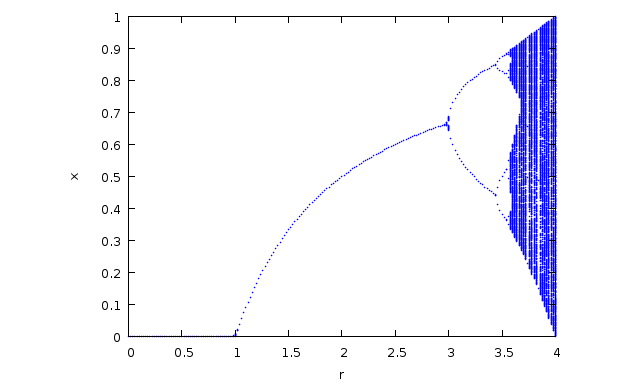
\includegraphics[width=9cm]{pic2.png}
    
\end{center}
\vspace{0.3cm}

De esta gráfica podemos sacar las mismas conclusiones que de la gráfica en la sección anterior, que las tasas de crecimiento entre 0.0 y 1.0 causan la extinción en el sistema, su atractor es 0.0, entre 1.0 y 2.9 tienden a un nivel de población estable, su atractor en un numero fijo. 

\begin{center}
	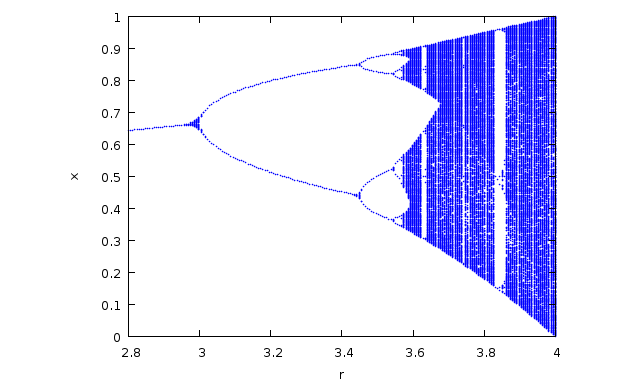
\includegraphics[width=9cm]{pic3.png}
    
\end{center}
\vspace{0.3cm}

Haciendo zoom entre 2.8 y 4 uno puede ver claramente que para tasas de crecimiento mas altos, estos tienen atractores extraños con varios valores, entre mas se acerca la tasa de crecimiento al 4, los atractores tienen mas valores.

\subsection{The Onset of Chaos}

Haciendo zoom a un espacio aun mas pequeño, de 3.7 a 3.9, obtenemos la siguiente gráfica:

\begin{center}
	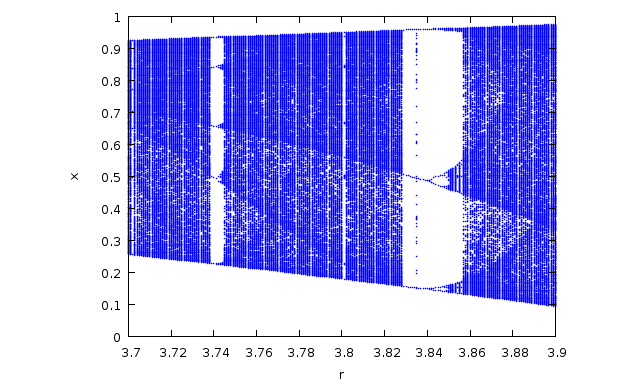
\includegraphics[width=9cm]{pic4.png}
    
\end{center}
\vspace{0.3cm}

Podemos que que hay mucho valores a los que pueden tender estas tasas de crecimiento, pero también podemos notar algo peculiar. Existen pequeñas secciones en estas tasas de crecimiento altas en que los actractores solo tienden a unos cuanto valores, pero rápidamente regresa al caos.

\subsection{Fractals and Strange Attractors}

Ahora veremos la pequeña sección entre 3.840 y 3.856 para la tasa de crecimiento y 0.45 y 0.55 para el nivel de la población:

\begin{center}
	\includegraphics[width=11cm]{pic5.png}
    (¡NOTA!)
\end{center}
\vspace{0.3cm}

Si hemos estado prestando atención, podemos notar que esta gráfica es prácticamente idéntica a otra que mostramos anteriormente, y si siguiéramos seleccionando secciones cada vez mas y mas pequeñas, seguiríamos encontrando este mismo patrón. 

Esto es porque los atractores extraños pueden ser caracterizados como fractales, los cuales tienen la misma estructura en cada escala.

\vspace{0.3cm}

Con un diagrama de fase podemos visualizar el valor de la población de la generación \textit{t+1} en el eje \textit{y}, contra su valor en \textit{t} en el eje \textit{x}.
Esto es porque si conocemos el valor de la población en \textit{t}, podemos conocerlo en \textit{t+1}.

\begin{center}
	\includegraphics[width=11cm]{pic6.png}
    (¡NOTA!)
\end{center}
\vspace{0.3cm}

Como podemos observar, para diferentes tasas de crecimiento se muestran sus atractores, solo uno para 2.9, cuatro para 3.5.
Veamos que pasa con tasas de población mas altas.

\begin{center}
	\includegraphics[width=11cm]{pic7.png}
    (¡NOTA!)
\end{center}
\vspace{0.3cm}

Estas gráficas forman parábolas, todas diferentes, dependiendo de su tasa de crecimiento. Para la gráfica de la derecha, con tasas de crecimiento entre 3.6 y 4.0, se puede decir que este es su \textit{Régimen Caótico}, que es el rango de parámetros, en este caso tasas de crecimiento, en el que el sistema se comporta de manera caótica.

Los atractores extraños suelen tener este tipo de formas, el sistema parece estar restringido de cierta manera, pero nunca se asienta en un punto o una oscilación constante, solo rebota entre diferentes valores de población sin repetir uno. 

\subsection{Chaos vs Randomness}

Los diagramas que acabamos de mostrar son \textit{diagramas de fase}, los cuales usan diferentes variables del sistema como sus dimensiones, cada punto en el espacio de estado es un posible estado del sistema.
Estos son muy útiles a la hora de mostrar el comportamiento de atractores extraños ya que gráficas datos de una dimensión en dos o tres dimensiones. En especial para diferenciar caos determinista de un comportamiento aleatorio.

\begin{center}
	\includegraphics[width=11cm]{pic8.png}
    (¡NOTA!)
\end{center}
\vspace{0.3cm}

Aquí, las dos lineas parecen tener comportamiento aleatorio cuando en realidad una de ellas representa diferentes valores de población para una tasa de crecimiento de 3.99. ES difícil diferenciar uno de otro de esta manera, por eso, veremos estos diagramas en dos y 3 dimensiones, para diferenciarlos.

\begin{center}
	\includegraphics[width=11cm]{pic9.png}
    (¡NOTA!)
\end{center}
\vspace{0.3cm}

Así podemos ver un patrón para nuestro caos determinista y distinguirlo de el comportamiento aleatorio que sigue sin tener forma.

\vspace{0.3cm}

Ahora, vamos a graficar el régimen caótico en 3-D:

\begin{center}
	\includegraphics[width=11cm]{pic10.png}
    (¡NOTA!)
\end{center}
\vspace{0.3cm}

Esta estructura muestra que en lo que un principio pensábamos que era comportamiento aleatorio, con nuestros mapas logísticos, en realidad es un caos determinista aperiódico, limitado por atractores extraños.

\subsection{The Butterfly Effect}

Los sistemas caóticos son MUY sensibles a sus condiciones iniciales, en sistemas con atractores extraños, condiciones iniciales cercanas tienden a divergir. Esto se vuelve un problema al simular sistemas caóticos reales, ya que algo como un error de redondeo puede afectar de manera significativa a la simulación con el paso del tiempo. 

Aquí se muestra un ejemplo de un modelo logístico con valores muy parecidos.

\begin{center}
	\includegraphics[width=11cm]{pic11.png}
    (¡NOTA!)
\end{center}
\vspace{0.3cm}

Los dos tienen la misma tasa de crecimiento, pero por una diferencia tan pequeña de 0.00001 en su valor inicial, después de la generación numero 30, parecen sistemas completamente diferentes.

A esto se le conoce come \textit{Efecto Mariposa}, el cual dice que algo tan pequeño como el aleteo de una mariposa puede causar eventos descomunales en el paso del tiempo. Esto quiere decir que eventos muy pequeños pueden tener repercusiones muy grandes a la larga.

\subsection{The Implications of Chaos}
Los sistemas caóticos se presentan en todo momento en todas partes, en todas las ciencias. Esto significa que nuestras predicciones (modelos o simulaciones) solo pueden llegar hasta cierto punto antes de divergir de la realidad. 



\section{Bilbiografía}

\begin{verbatim}
Gboeing, A. (2016, October 21). Chaos Theory and the Logistic Map. 
Retrieved from http://geoffboeing.com/2015/03/chaos-theory-logistic-map/ 
\end{verbatim}
%http://geoffboeing.com/2015/03/chaos-theory-logistic-map/

\begin{verbatim}
https://arxiv.org/pdf/1301.3240.pdf
\end{verbatim}
%https://arxiv.org/pdf/1301.3240.pdf

\vspace{0.3cm}

\section*{Nota}
Todas las imágenes que tienen escrito \textit{(¡NOTA!)} debajo de ellas son capturas de pantalla (imagenes: 1,5-11), ya que no pude reproducir esas pero las quería poner para complementar el reporte. 

\end{document}